\section{Theory}

	The dielectric constant of a material, also known as its permittivity $(\epsilon)$, is a complicated number whose real portion, $(\epsilon')$, represents energy stored and whose imaginary part, $(\epsilon'')$, represents energy lost. It may alternatively be described as the difference between the capacitance of a capacitor that contains a dielectric and a capacitor that is similar but empty. The material's capacity to release the absorbed electromagnetic energy is represented by the dielectric loss factor, $(\epsilon'')$. EM waves tend to penetrate samples less deeply the greater their dissipation capacity.

	The real part of permittivity depends on the polarizability of the material. The total polarizability can be separated into four parts:\\
	\begin{enumerate}
		\item \textbf{Electronic Polarization:} because of the nucleus's displacement with respect to the electron cloud that surrounds it. The displacement induces charges on the atom, leading to the development of a dipole moment. The mechanism operates quickly and continues to function up to optical frequencies ($10^{13}-10^{15}$ Hz). Takes place in neutral atoms.\\
		\item \textbf{Ionic Polarization:} It happens in solids with ionic bonding when the net dipole is zero because of the crystal symmetry. Ions are moved out of their equilibrium position by an external field, which induces a dipole moment. This mechanism operates at low frequencies and is comparatively sluggish. Only losses are introduced into a system through ionic conduction.\\
		\item \textbf{Dipolar/Orientation Polarization:} It happens in molecules with an ongoing dipole moment. When an external electric field is introduced, randomly distributed dipoles align, increasing the overall polarization. This process operates below $10^9$ Hz and is slower than ionic polarization.\\
		\item \textbf{Space Charge Polarization:} This process happens when translating charge carriers become caught at the interfaces of these heterogeneous systems, such as in composite materials or when segregation happens in a material with incompatible chemical sequences. Positive and negative space charges arise in the bulk of the material or at the interfaces between various materials as a result of the separation of mobile charge carriers under an electric field. This method works well in the audio frequency spectrum, because charge carriers require time to build up at interfaces.
	\end{enumerate}
	\begin{figure}[H]
		\centering
		\label{fig:1}
		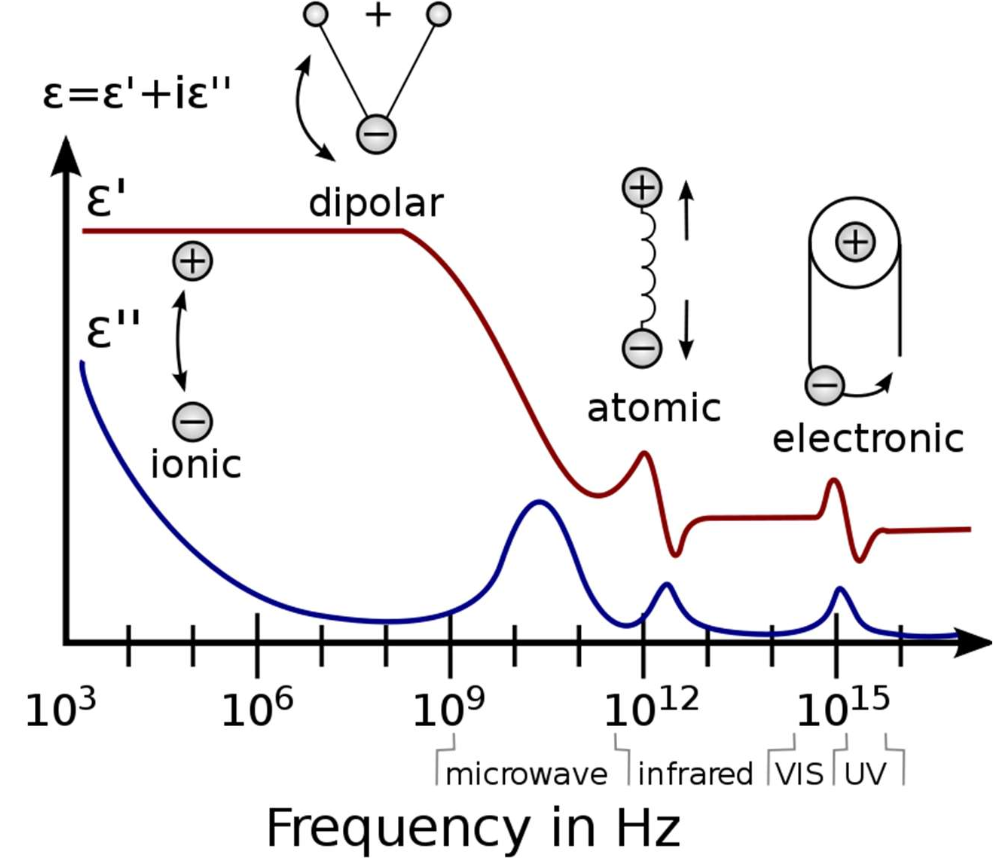
\includegraphics[width=0.8\columnwidth]{images/t1.png}
		\caption{Real and Imaginary part of permittivity (dielectric constant) as a function of frequency}
	\end{figure}
	
	\subsection*{Variation of the dielectric constant\\
	with alternating fields}
		We are aware that an electric field causes a dielectric to become polarised. In a field that changes direction, the polarisation will likewise change direction to match the new field. The transfer of charges or the rotation of dipoles requires time, therefore this cannot happen instantly.

		The average dipole orientation adjusts over a particular period of time known as the relaxation time when the field is altered. Around $10^{-11}$ s is the typical relaxation time. As a result, if the electric field alternates directions at a frequency greater than $10^{11}$ Hz, the polarization mechanism no longer contributes to the polarisation of the dielectric because the dipole orientation is unable to ``keep up" with the alternating field and cannot maintain its alignment with it.
		
		Only the fastest mechanism (electronic polarization) contributes, as the slower mechanisms (ionic,
		orientational, and space charge) cannot follow rapid field changes. The polarization process stops helping to polarise the dielectric at higher frequencies because the flow of charge cannot keep up with the alternating field. As frequency rises, the material's net polarisation decreases because it no longer contributes to the overall polarisation, and as a result, its dielectric constant decreases.

	The ratio $\epsilon''/\epsilon'$ (loss tangent or $\tan \delta$) is a crucial parameter in microwave heating, as it quantifies the efficiency of converting microwave energy into heat. A higher $\epsilon''/\epsilon'$ means more effective heating. 
	% The loss tangent, $\tan \delta$, is defined as,

	% \begin{align}
	% 	\tan \delta = \frac{\epsilon}{}
	% \end{align}


	\subsection*{Variation of the dielectric constant with Temperature}
		The electrostatic forces generated by the field cause the molecules to rotate and align with it. However, due to the thermal motion the molecules are experiencing, not all of them are perfectly aligned with the field.

		Because the molecules have more thermal energy as the temperature rises, the amplitude of random thermal motion also increases. As a result, the molecules are less tightly aligned with one another, which results in less orientation polarisation of the material and a lower dielectric constant. This indicates that the range of departure from a perfect alignment with the external electric field is higher.

		As the temperature is reduced, the dielectric constant does not, however, rise continuously. At phase boundaries, the dielectric constant will abruptly alter. This is because during a phase transition, the structure alters, and as we've shown above, the structure has a significant impact on the dielectric constant.
		
	\subsection{The Dissipation factor}

	To quantify the broadening of the phase
	transition, the diffuseness parameter, $\delta$ can be written as the slope of the $\log(\frac{1}{\epsilon}-\frac{1}{\epsilon_C})$ vs. $\log(\frac{1}{T}-\frac{1}{T_C})$ plot,
	
	\begin{align}
		\log\left(\frac{1}{\epsilon}-\frac{1}{\epsilon_c}\right) = \delta \cdot \log\left(\frac{1}{T}-\frac{1}{T_C}\right)
	\end{align}
	
	where $\epsilon$ is the dielectric constant at a temperatures $T > T_C$, ${\epsilon_C}$  is the maximum value of the dielectric constant at the Curie temperature $T_C$. 

\subsection{Properties of BaTiO$_3$}

	\textit{Perovskite} substances like Barium Titanate or CaTiO$_3$ have a relatively high dielectric constant at ambient temperature. In the perovskites crystal structure, while B-site cations sit in the centre of the body, A-site cations take up the corners of a cube. On the faces are three oxygen atoms per cell.

	\begin{figure}[H]
		\centering
		\label{fig:2}
		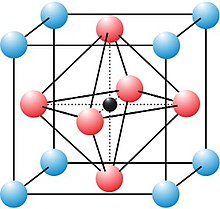
\includegraphics[width=0.4\columnwidth]{images/t3.jpg}
		\caption{Perovskite Structure}
	\end{figure}

	The lattice constant of perovskites is typically around 4 $\angstrom$ due to the rigid oxygen octahedral network and the oxygen ionic radius of 1.35 $\angstrom$. A key advantage of the perovskite structure is the ability to substitute various cations on the A and B sites without significantly altering the structure. This allows for the formation of complete solid solutions, enabling the manipulation of material properties like Curie Temperature and dielectric constant through small cation substitutions.

	Below and beyond its $120^\circ$C Curie point, barium titanate exhibits a paraelectric cubic phase and a ferroelectric tetragonal phase respectively. The contaminants in a sample and the synthesis method have an impact on the Curie point temperature of that sample. 
	
	In the paraelectric cubic phase, the centres of positive charges (Ba$^{2+}$, Ti$^{4+}$) coincide with the centres of negative charges (O$^{2-}$ ion). However, when the temperature is cooled below $T_C$, we observe a tetragonal phase in which the centres of the Ba$^{2+}$ and Ti$^{4+}$ ions are dislocated in relation to the O$^{2-}$ ion, resulting in the formation of electric dipoles. As a result, the of BaTiO$_3$ rises until $T_C$ and reaches its maximum value at $T = T_C$ due to the divergence of susceptibility at that point. The spontaneous polarization vanishes as the centers of positive and
	negative charges coincide. After crossing this temperature it starts decreasing due to the formation of the cubic phase.

% ======================================================================================
\section{Experimental Setup}

\subsection*{Apparatus}

\begin{enumerate}
    \item BaTiO$_3$ capacitor sample
    \item Standard Multilayer Ceramic Capacitor
    \item Disc Ceramic Capacitor
    \item Aluminium plate
    \item Oscilloscope
    \item Probe Arrangement
    \item Setup consisting of Schering Bridge
\end{enumerate}

\begin{figure}[H]
	\centering
	\label{fig:setup}
	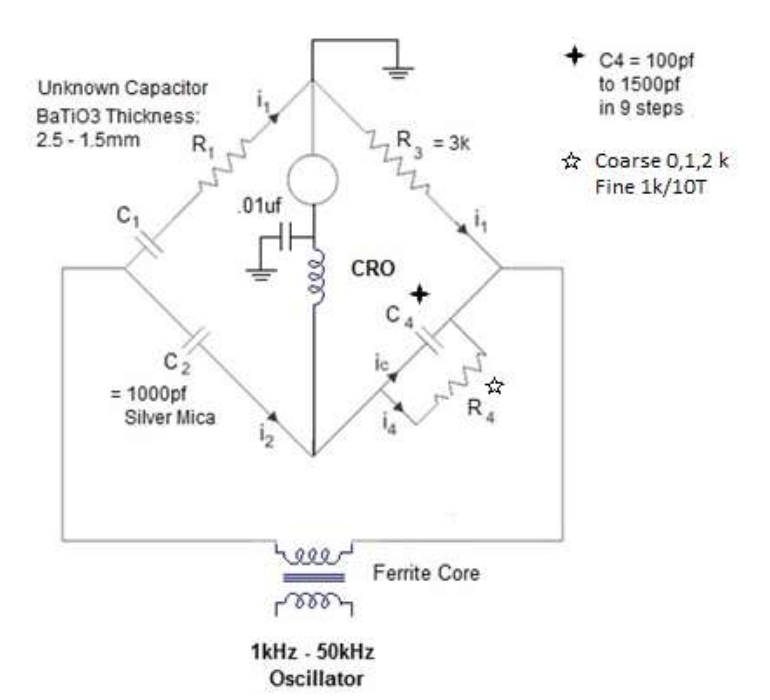
\includegraphics[width=0.7\columnwidth]{images/t5.png}
	\caption{Schering Bridge}
\end{figure}

In the first part of the experiment, we study the frequency dependence of dielectric constant. The main unit is used in the setup to measure capacitance at frequencies between 1kHz and 50kHz. A built-in oscillator and a Schering Bridge (\hyperref[fig:setup]{Fig. 3}) are used to accomplish this. Here, the value of the unknown capacitance (BaTiO$_3$), $C_1$ is to be ascertained by using $R_1$ as a series electrical resistance. $C_2$ is a typical 1000 pf silver mica capacitor. $C_4$ is a variable capacitor with Coarse and Fine adjustment. The metal film resistance, $R_3$, is 1.0 k$\Omega$. $R_4$ is a variable resistance with Coarse and Fine 1k/10T potentiometers in series and parallel to $C_4$, respectively. 

The impedances in each arm are given by,
\begin{align*}
	Z_1 &= R_1 + \frac{1}{j\omega C_1}\\
	Z_2 &=  \frac{1}{j\omega C_2}\\
	Z_3 &= R_3\\
	Z_4 &= \frac{1}{\frac{1}{R_4} + j\omega C_4}\\
\end{align*}

From the bridge balance condition we get:

\begin{align}
	Z_1Z_4 &= Z_2Z_3 \nonumber\\
	\implies R_1&=\frac{R_3 C_4}{C_2}\\
	\text{and, }C_1&=\frac{R_4 C_2}{R_3}
\end{align}

From these, the dielectric constant $\epsilon$ can be calculated as

\begin{align}
	\epsilon = \frac{C_1}{C_0}
\end{align}

where $C_0$ is the standard capacitance value of the material used, $C_0 = \epsilon_0 A/d$. Here $C_1$ is the unknown capacitor and $R_1$ is the equivalent series resistance reflecting losses. The loss factor (dissipation factor) can be defined as:
\begin{align}
	\tan\delta=\frac{\epsilon'}{\epsilon''}
\end{align}

And from setup it can be calculated that,
\begin{align}
	\tan\delta=\omega C_1r_1 = 2\pi fC_1R_1
\end{align}